\documentclass[a4paper,12pt]{article}
\usepackage[utf8]{inputenc}
\usepackage{amssymb}
\usepackage{amsmath}
\usepackage{tikz}
\usetikzlibrary{arrows,calc,decorations.pathreplacing,fadings,intersections}
\usetikzlibrary{external}

\begin{document}

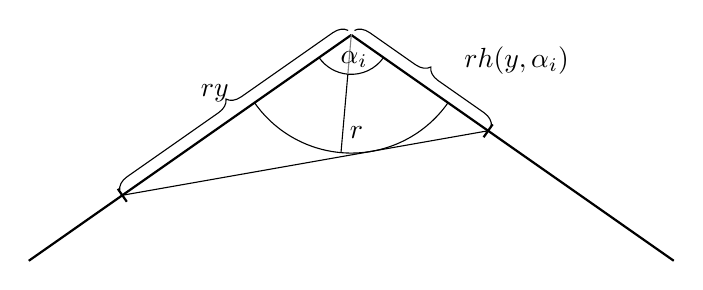
\begin{tikzpicture}[scale=.5,rotate=-35]
	\draw[white,name path=secondedge] (0,0) -- (10,0);
	\draw[thick] (0,0) -- (10,0);
	\draw[white, name path=firstedge] (0,0) -- ({10*cos(250)},{10*sin(250)});
	\draw[thick] (0,0) -- ({10*cos(250)},{10*sin(250)});
	\draw (1,0) arc[start angle=360, end angle=250, radius=1];
	\draw (3,0) arc[start angle=360, end angle=250, radius=3];
	\draw[black!50] ({0*cos(300)},{0*sin(300)}) -- ({1*cos(300)},{1*sin(300)});
	\draw ({1*cos(300)},{1*sin(300)}) -- ({3*cos(300)},{3*sin(300)}) node[near end,xshift=5pt]{$r$};
	\node at (0,0) [xshift=1pt,yshift=-9pt] {$\alpha_i$};

	\begin{scope}
		\clip (0,0)--({10*cos(250)},{10*sin(250)})--(10,0)--(0,0);
		\draw[name path=someline] ({3*cos(315)	+10*cos(225)},{3*sin(315)+10*sin(225)}) -- ({3*cos(315)	-10*cos(225)},{3*sin(315)-10*sin(225)});
		\fill [name intersections={of=someline and firstedge, by=t}] (t) circle (.001);
		\fill [name intersections={of=someline and secondedge, by=s}] (s) circle (.001);
	\end{scope}
	\draw[thick] ($(t)-({.2*cos(340)},{.2*sin(340)})$) --($(t)+({.2*cos(340)},{.2*sin(340)})$);
	\draw[decorate,decoration={brace,amplitude=5pt,raise=2pt,mirror}] (0,0) -- ($(t)$) node [midway,xshift=-8pt,yshift=8pt]{$ry$};
	\draw[decorate,decoration={brace,amplitude=5pt,raise=2pt}] (0,0) -- ($(s)$) node [midway,xshift=35pt,yshift=8pt]{$rh(y,\alpha_{i})$};
	\draw[thick] ($(s)-({.2*cos(90)},{.2*sin(90)})$) --($(s)+({.2*cos(90)},{.2*sin(90)})$);
\end{tikzpicture}

\end{document}